\appendix
\section{Appendix}

\subsection{Ethics}
This work does not raise any ethical issues and 
is determined to be non-human subjects research by our university's
Institutional Review Board.  The model of deployment is very much akin to a
``RIPE Atlas'' model, a longstanding mode for deploying measurement probes in
access networks.

\subsection{Resolvers}\label{sec:resolvers}
\begin{small}
\begin{itemize}
\item anycast.dns.nextdns.io
\item unicast.uncensoreddns.org
\item doh.ffmuc.net
\item jp.tiar.app
\item dns.therifleman.name
\item doh.pub
\item dns10.quad9.net
\item dns.adguard.com
\item doh.mullvad.net
\item dns12.quad9.net
\item dns-unfiltered.adguard.com
\item dns.alidns.com
\item helios.plan9-dns.com
\item dns1.ryan-palmer.com
\item dns.digitale-gesellschaft.ch
\item chewbacca.meganerd.nl
\item ordns.he.net
\item dns11.quad9.net
\item anycast.uncensoreddns.org
\item doh.libredns.gr
\item dns.brahma.world
\item dns.switch.ch
\item dns-doh-no-safe-search.dnsforfamily.com
\item ibksturm.synology.me
\item kronos.plan9-dns.com
\item dns-family.adguard.com
\item freedns.controld.com
\item dnsforge.de
\item dns-doh.dnsforfamily.com
\item public.dns.iij.jp
\item family.cloudflare-dns.com
\item dns.google
\item v.dnscrypt.uk
\item doh.dnscrypt.uk
\item doh.safesurfer.io
\item doh.la.ahadns.net
\item doh.tiar.app
\item doh.sb
\item doh-2.seby.io
\item dns.twnic.tw
\item dns.njal.la
\item pluton.plan9-dns.com
\item doh.seby.io
\item dns.quad9.net
\item dns.digitalsize.net
\item dns9.quad9.net
\item dohtrial.att.net
\item doh.nl.ahadns.net
\item adblock.doh.mullvad.net
\item adl.adfilter.net
\item per.adfilter.net
\item syd.adfilter.net
\item dns.nextdns.io
\item dns0.eu
\item doh.360.cn
\item open.dns0.eu
\item dnslow.me
\item kids.dns0.eu
\item pdns.itxe.net
\item security.cloudflare-dns.com
\item sby-doh.limotelu.org
\item dns.bebasid.com
\item 1dot1dot1dot1.cloudflare-dns.com
\item antivirus.bebasid.com
\item odoh-target-noads.alekberg.net
\item odoh-target-se.alekberg.net
\item odoh-target-noads-se.alekberg.net
\item odoh-target.alekberg.net
\item dnsse-noads.alekberg.net
\item dnsse.alekberg.net
\item family.puredns.org
\item dnsnl.alekberg.net
\item dnsnl-noads.alekberg.net
\item puredns.org
\item dns.circl.lu
\end{itemize}
\end{small}

\subsection{Response Time Measurements}

\begin{figure*}[h!]
\centering
\begin{subfigure}[b]{0.35\textwidth}
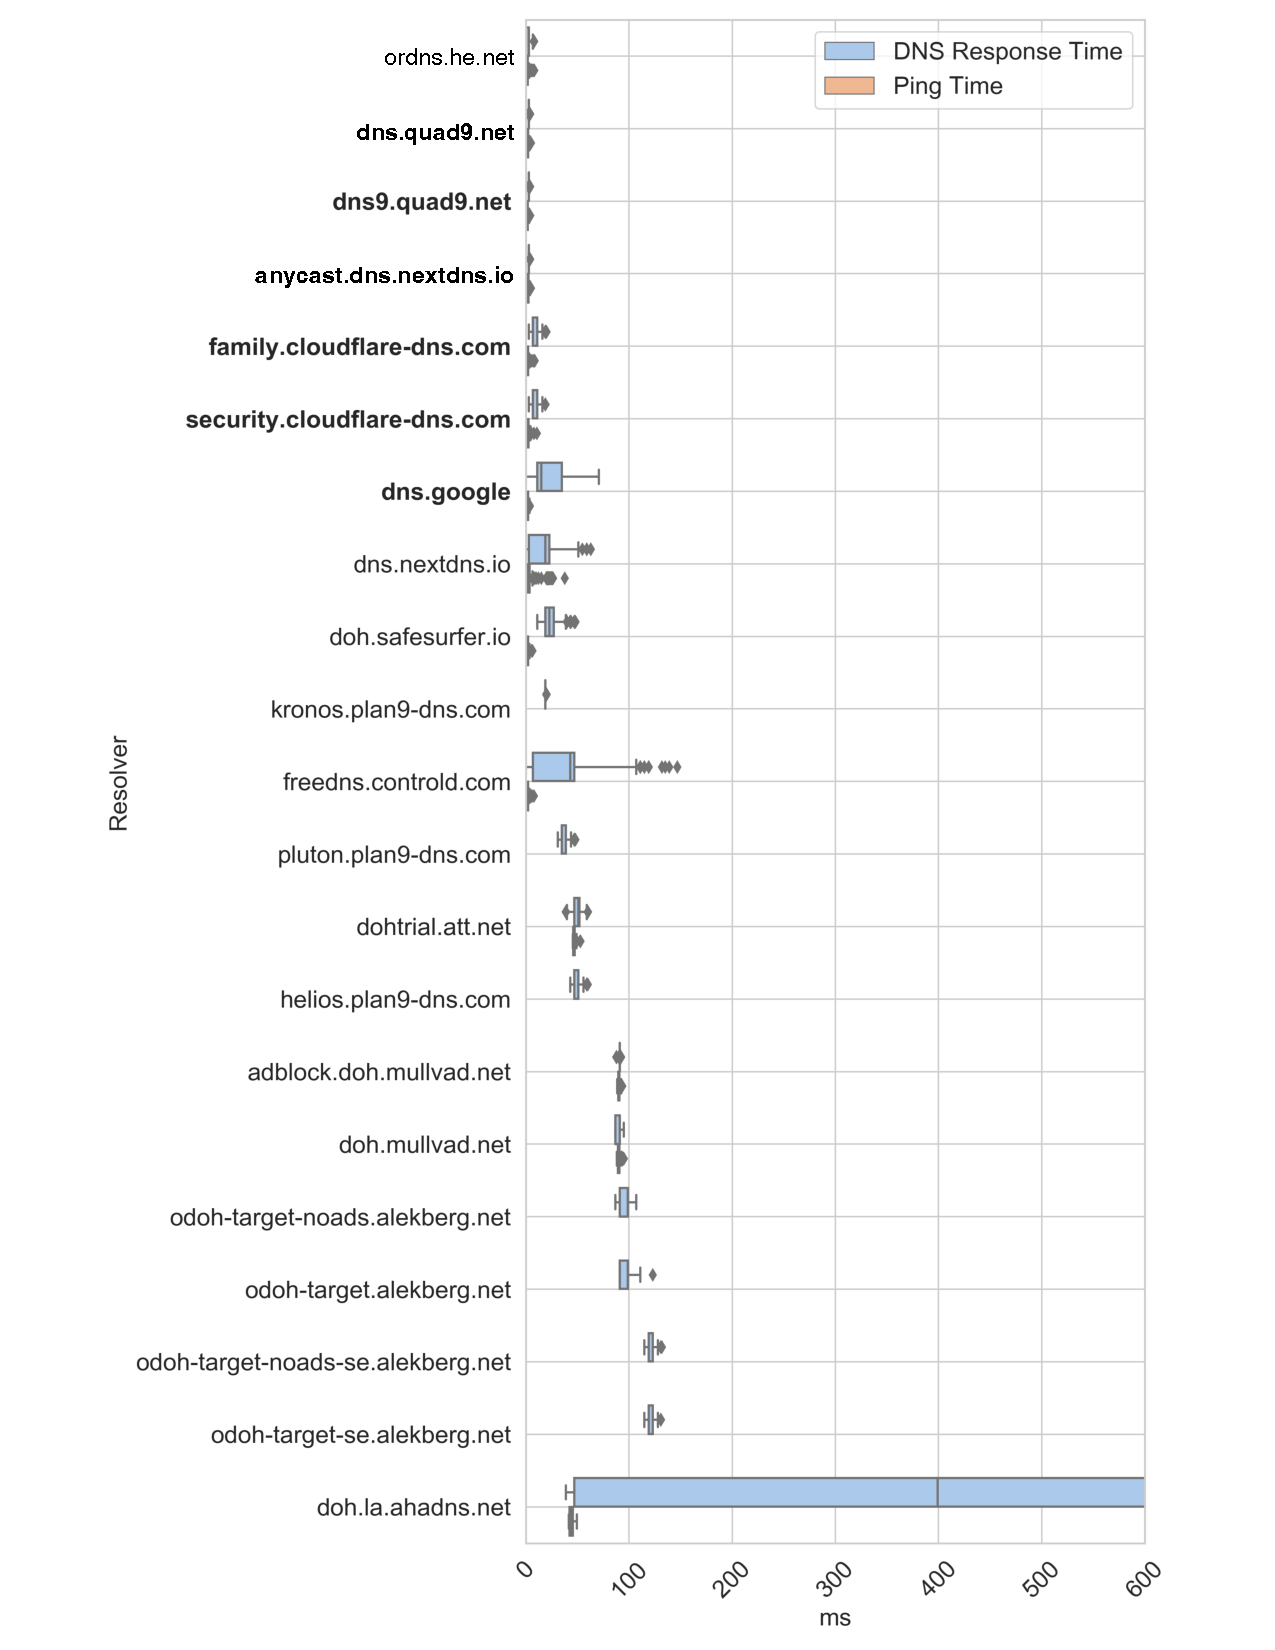
\includegraphics[width=\textwidth]{figures/poah_NA.pdf}
    \caption{U.S. Home Networks (Local)}
\end{subfigure}
%
\begin{subfigure}[b]{0.35\textwidth}
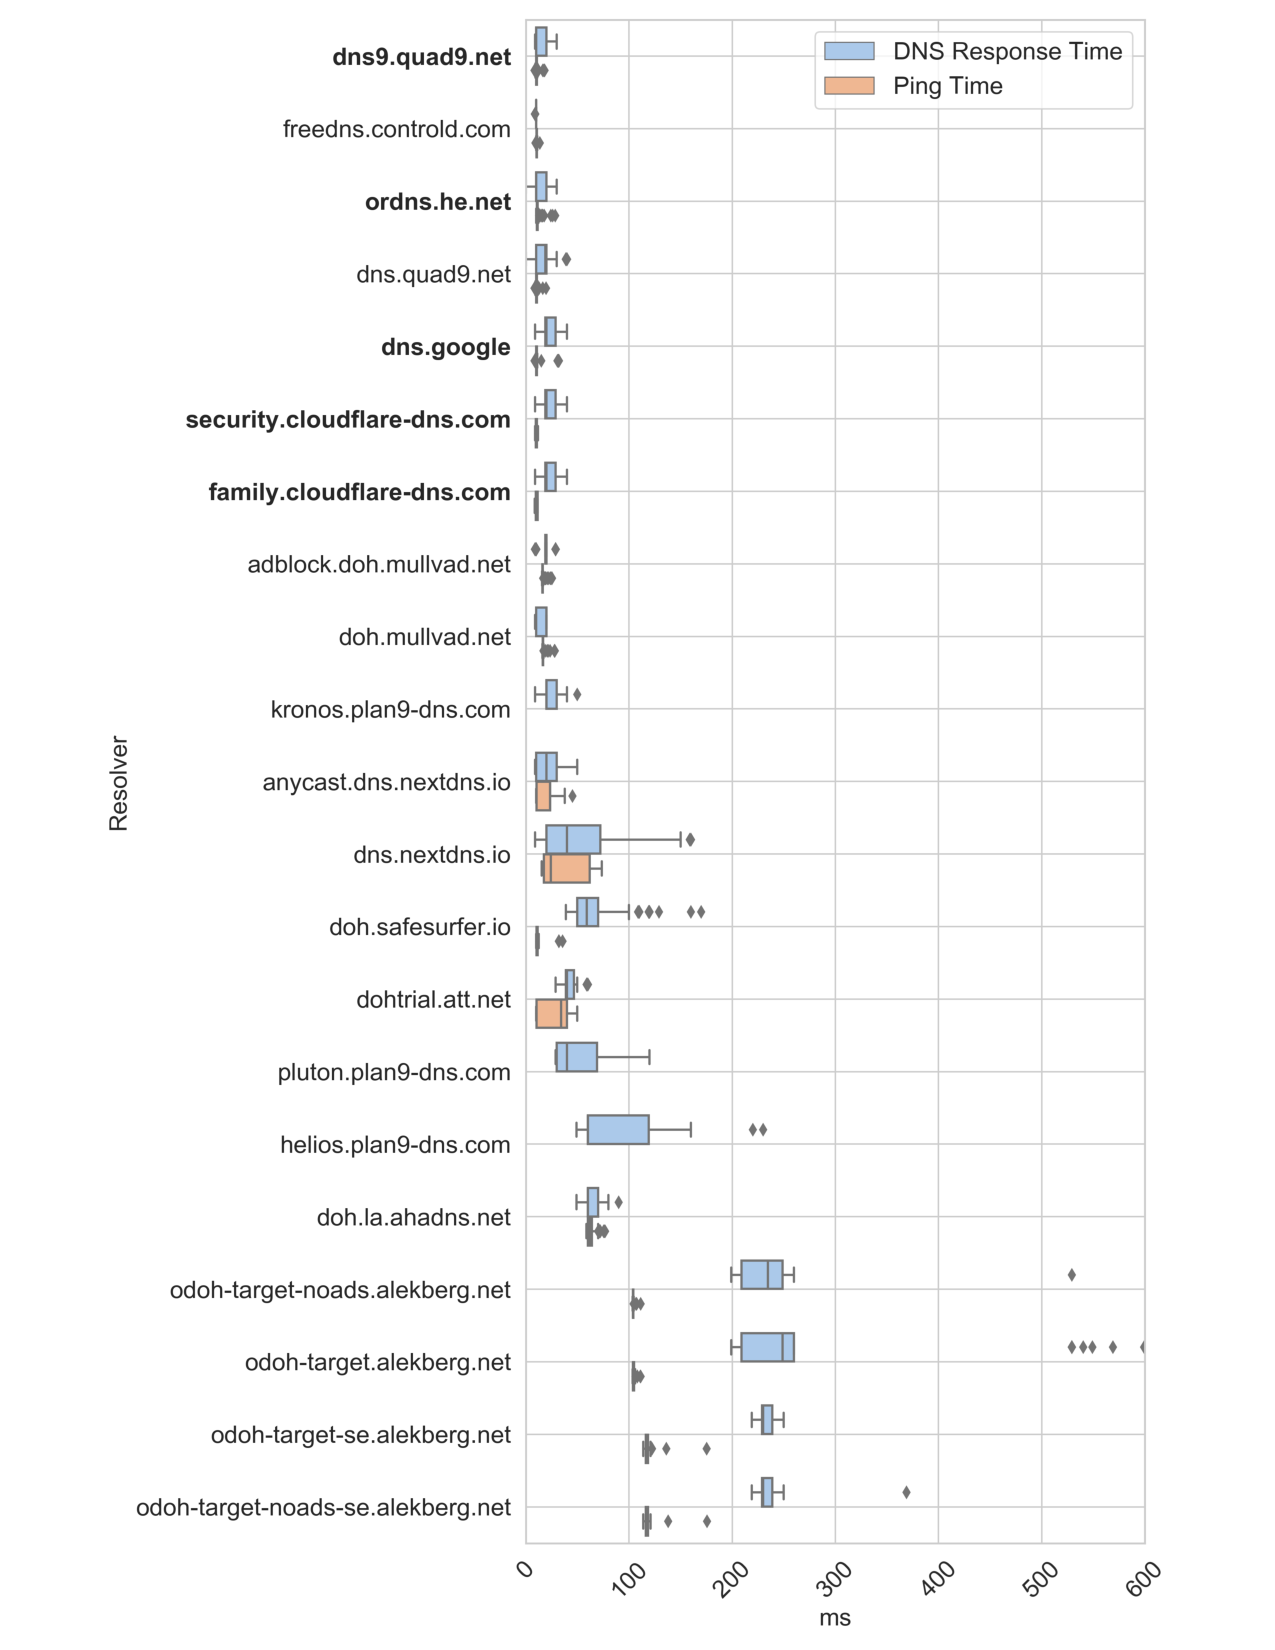
\includegraphics[width=\textwidth]{figures/ohio_NA.pdf}
    \caption{Ohio EC2 (Local).}
\end{subfigure}
%
\hfill \\
\begin{subfigure}[b]{0.35\textwidth}
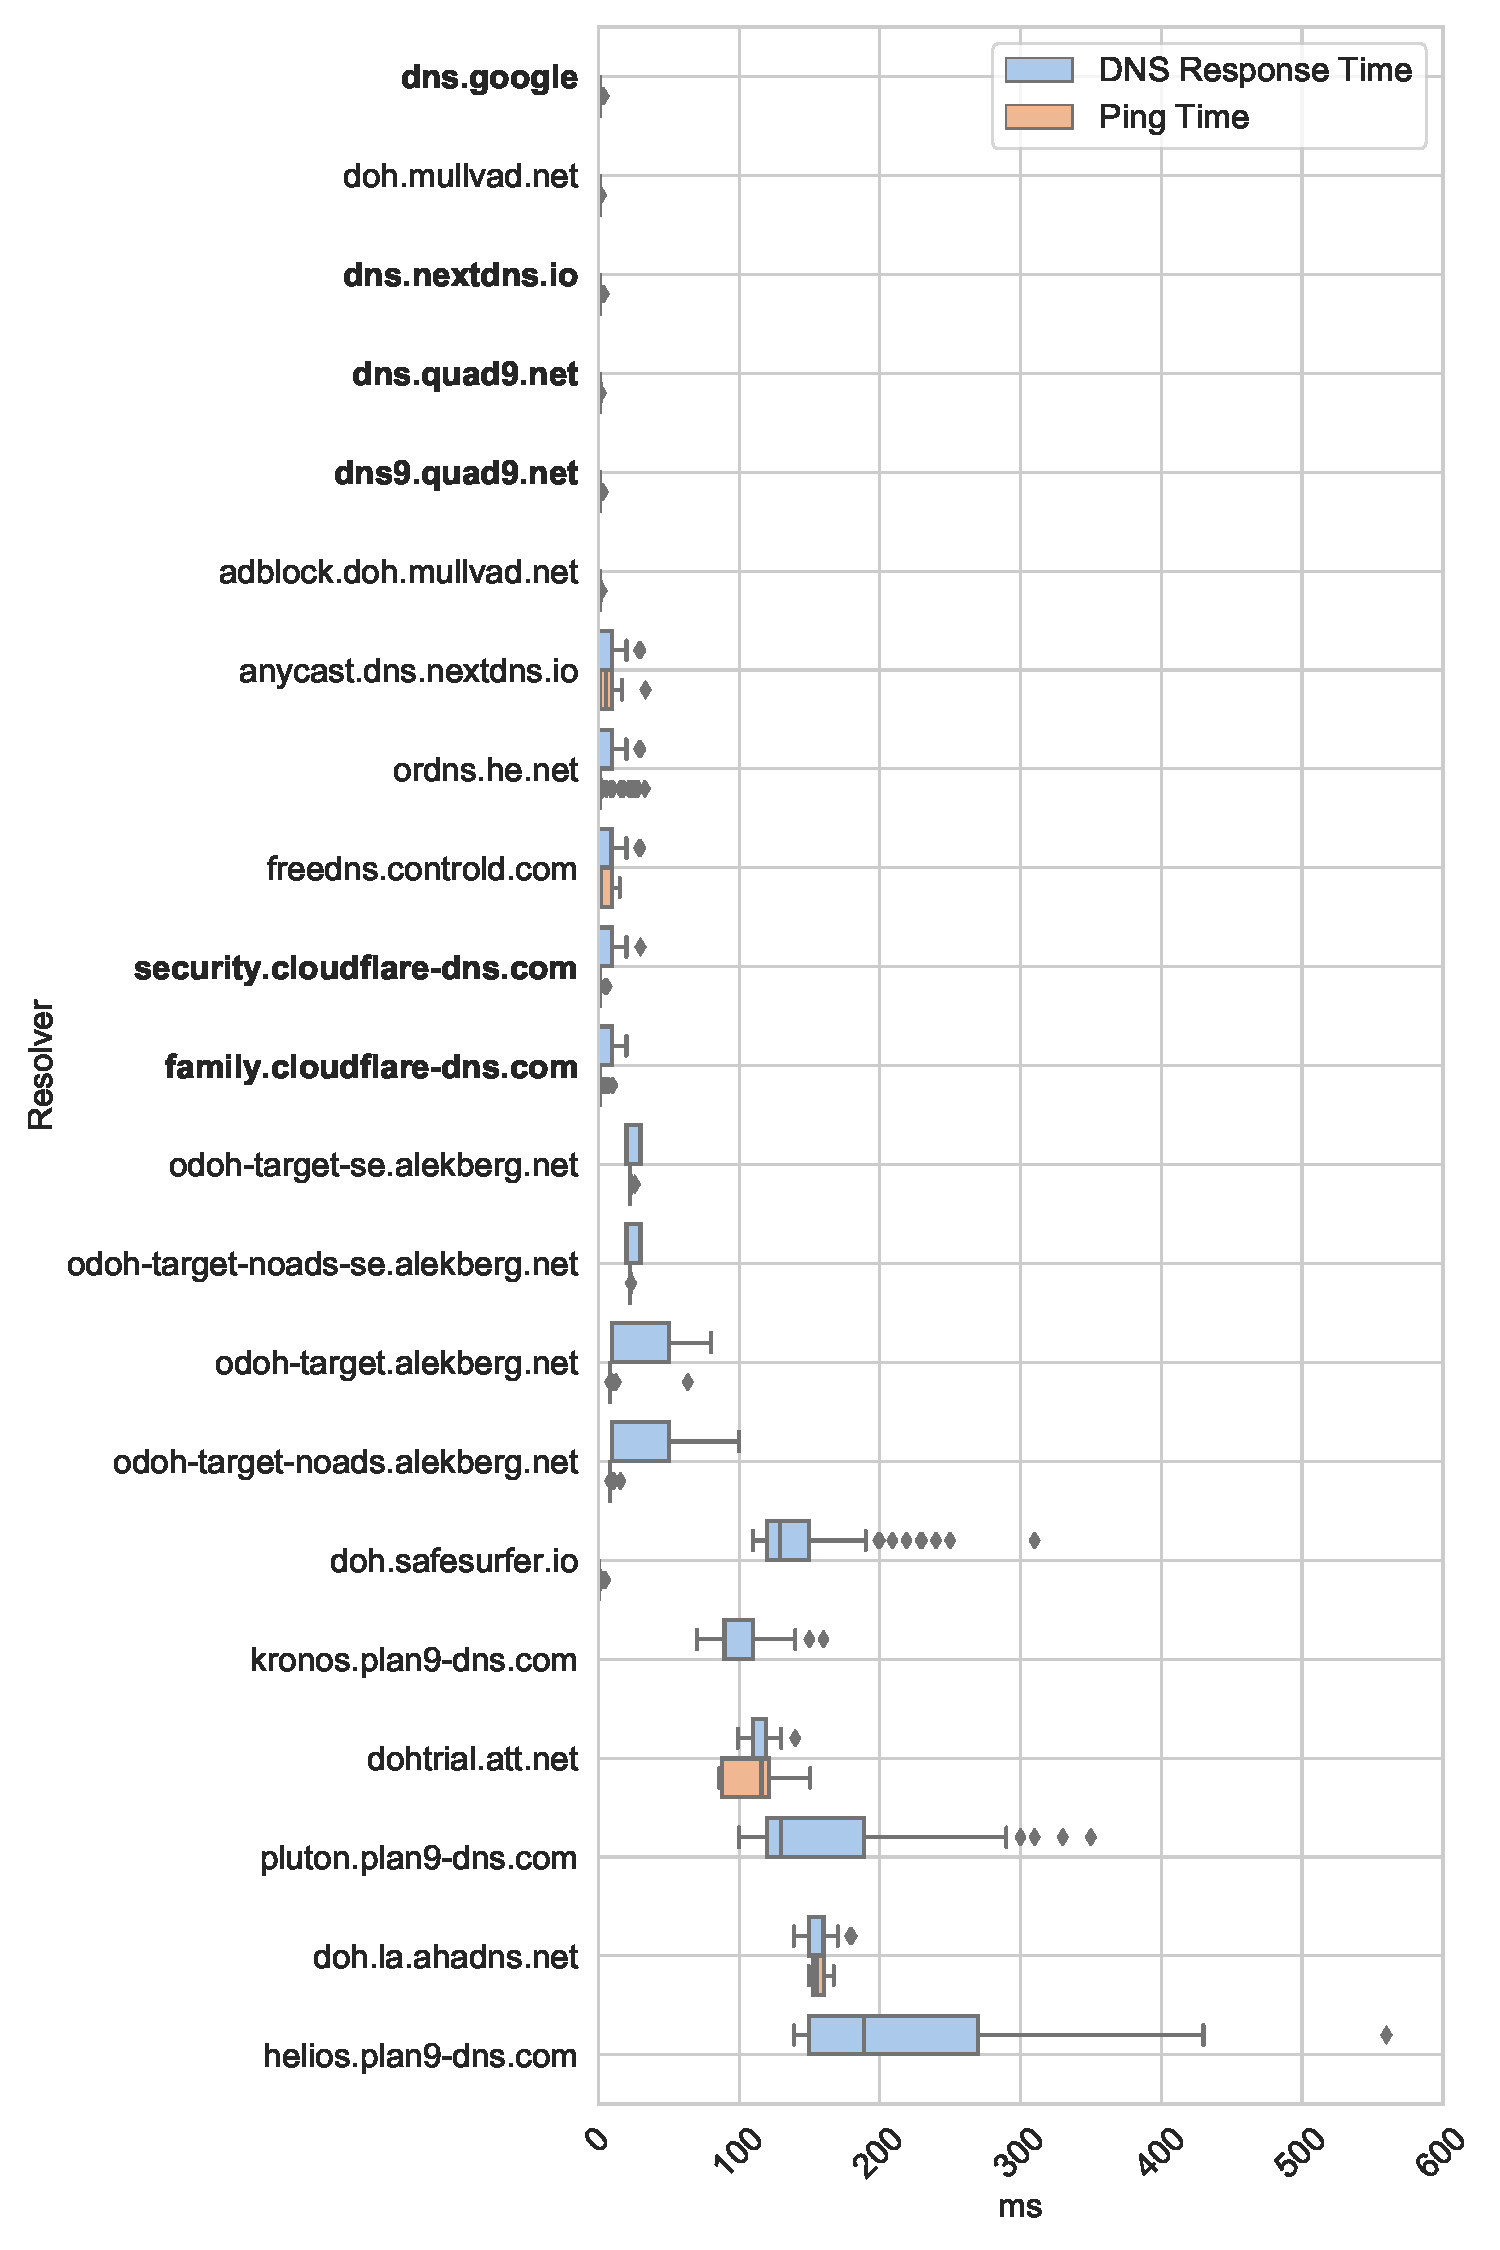
\includegraphics[width=\textwidth]{figures/frankfurt_NA.pdf}
    \caption{Frankfurt EC2.}
\end{subfigure}
%
\begin{subfigure}[b]{0.35\textwidth}
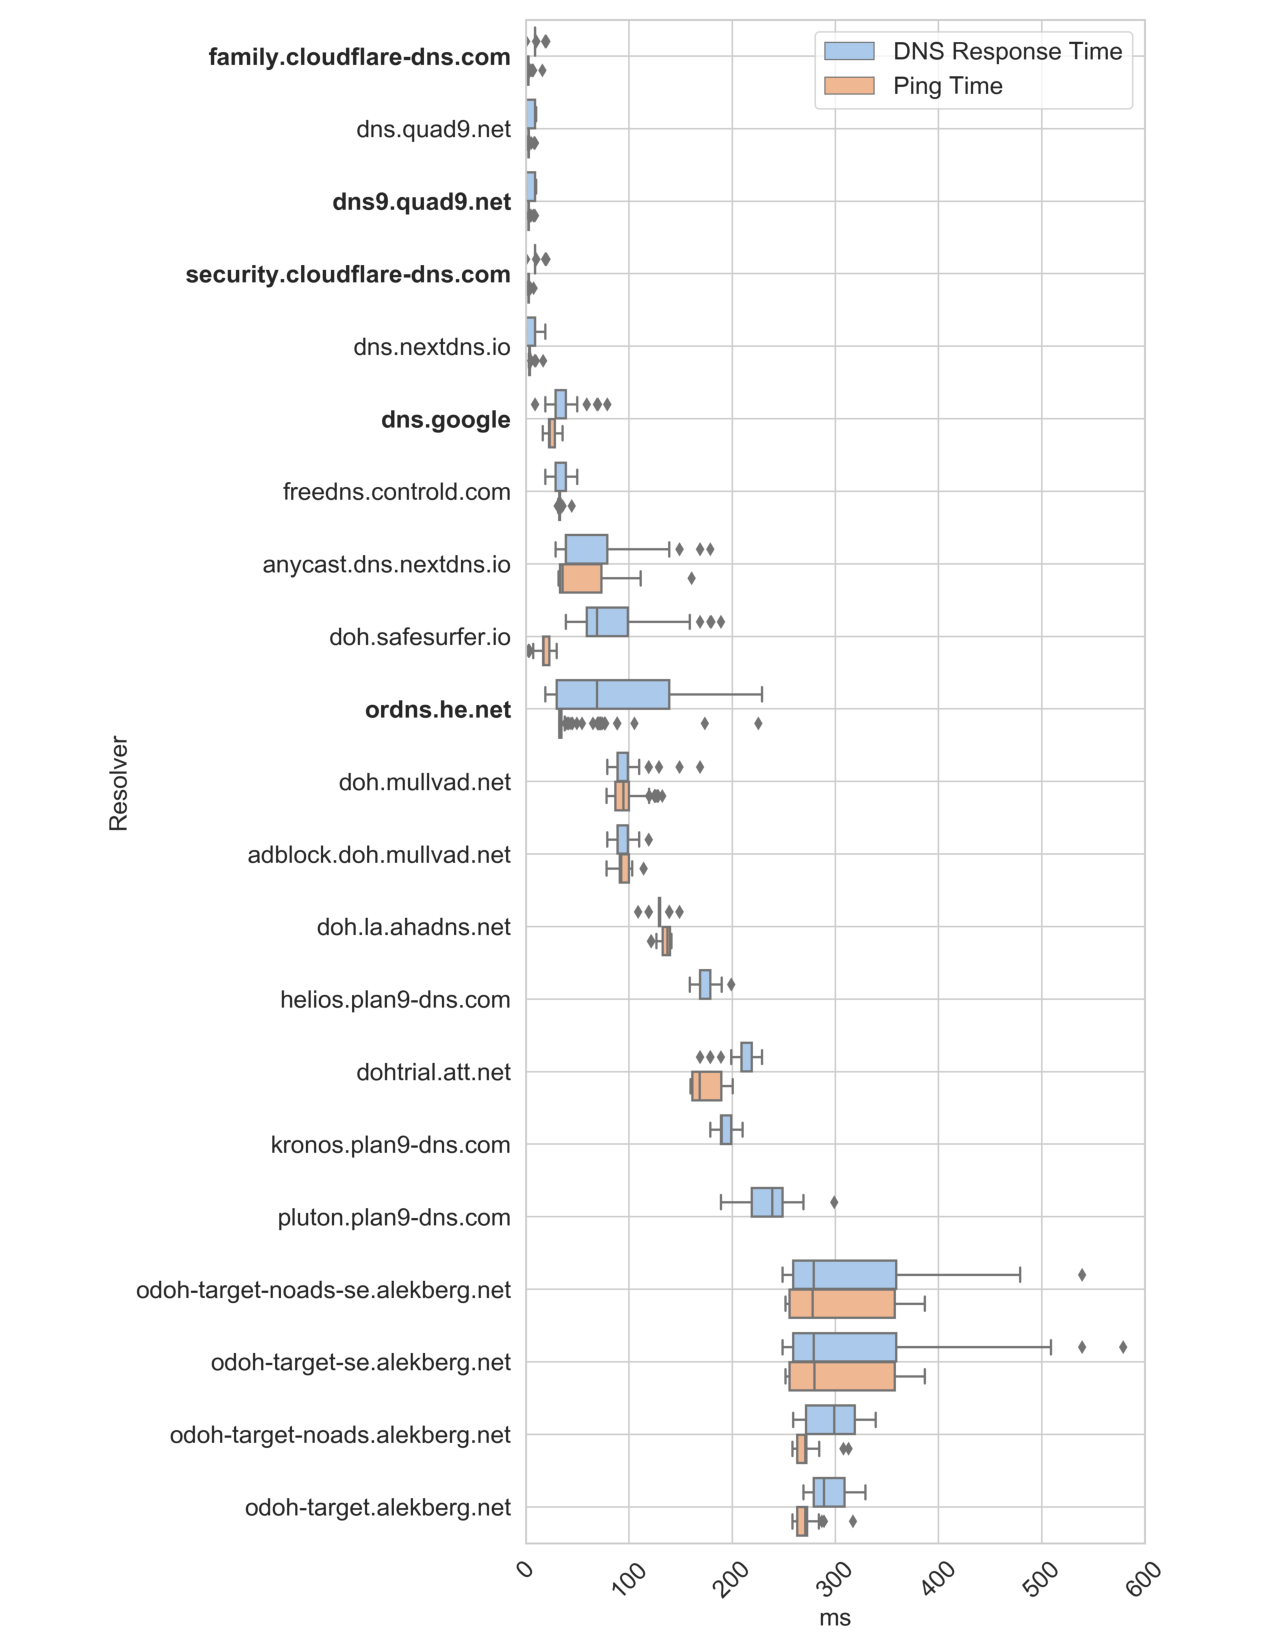
\includegraphics[width=\textwidth]{figures/seoul_NA.pdf}
\caption{Seoul EC2.}
\end{subfigure}
\caption{The DNS response time and ICMP ping time distributions for
    encrypted DNS resolvers located in North America, measured from global vantage points.
    Mainstream resolvers are shown in boldface across all three
    sub-figures.}
\label{fig:dns-NA}
\end{figure*}

\begin{figure*}[h!]
\centering
%
\begin{subfigure}[b]{0.4\textwidth}
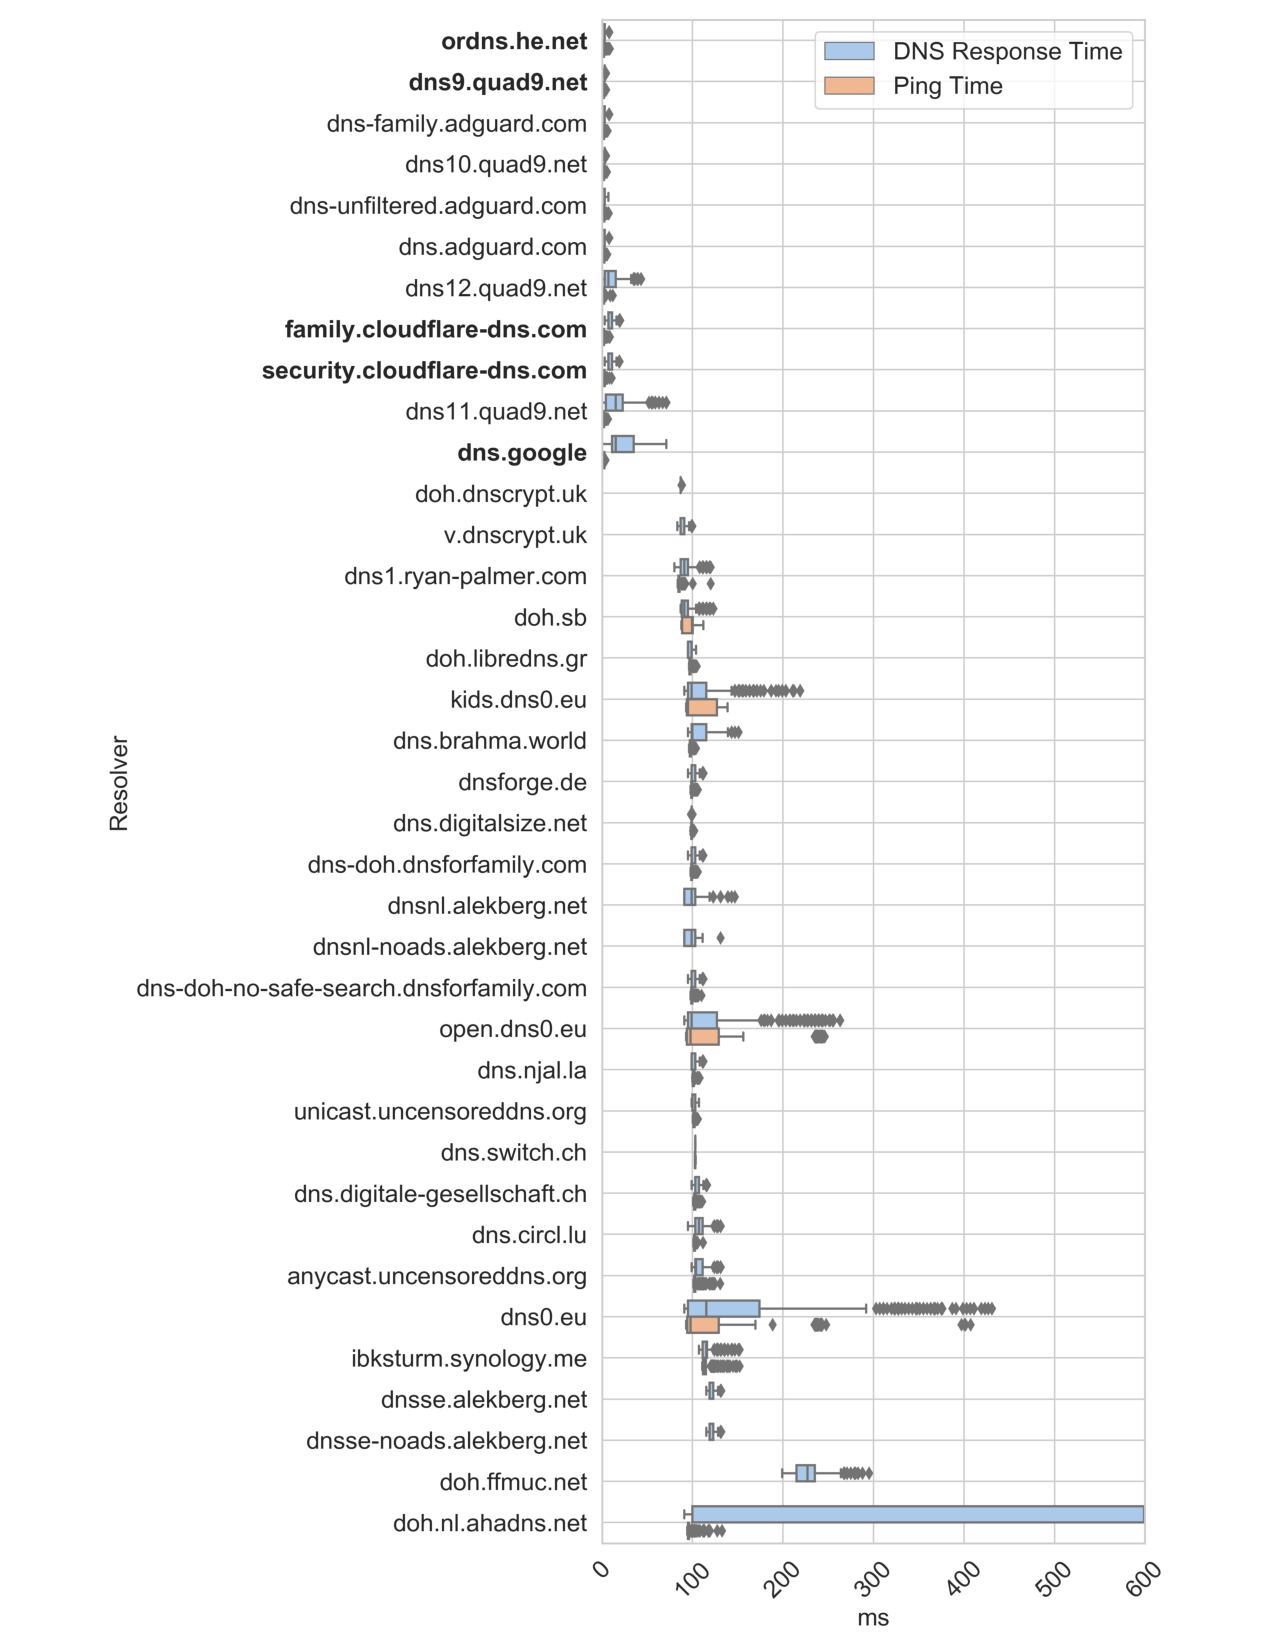
\includegraphics[width=\textwidth]{figures/poah_europe.pdf}
\caption{U.S. Home Networks.}
\end{subfigure}
%
\begin{subfigure}[b]{0.4\textwidth}
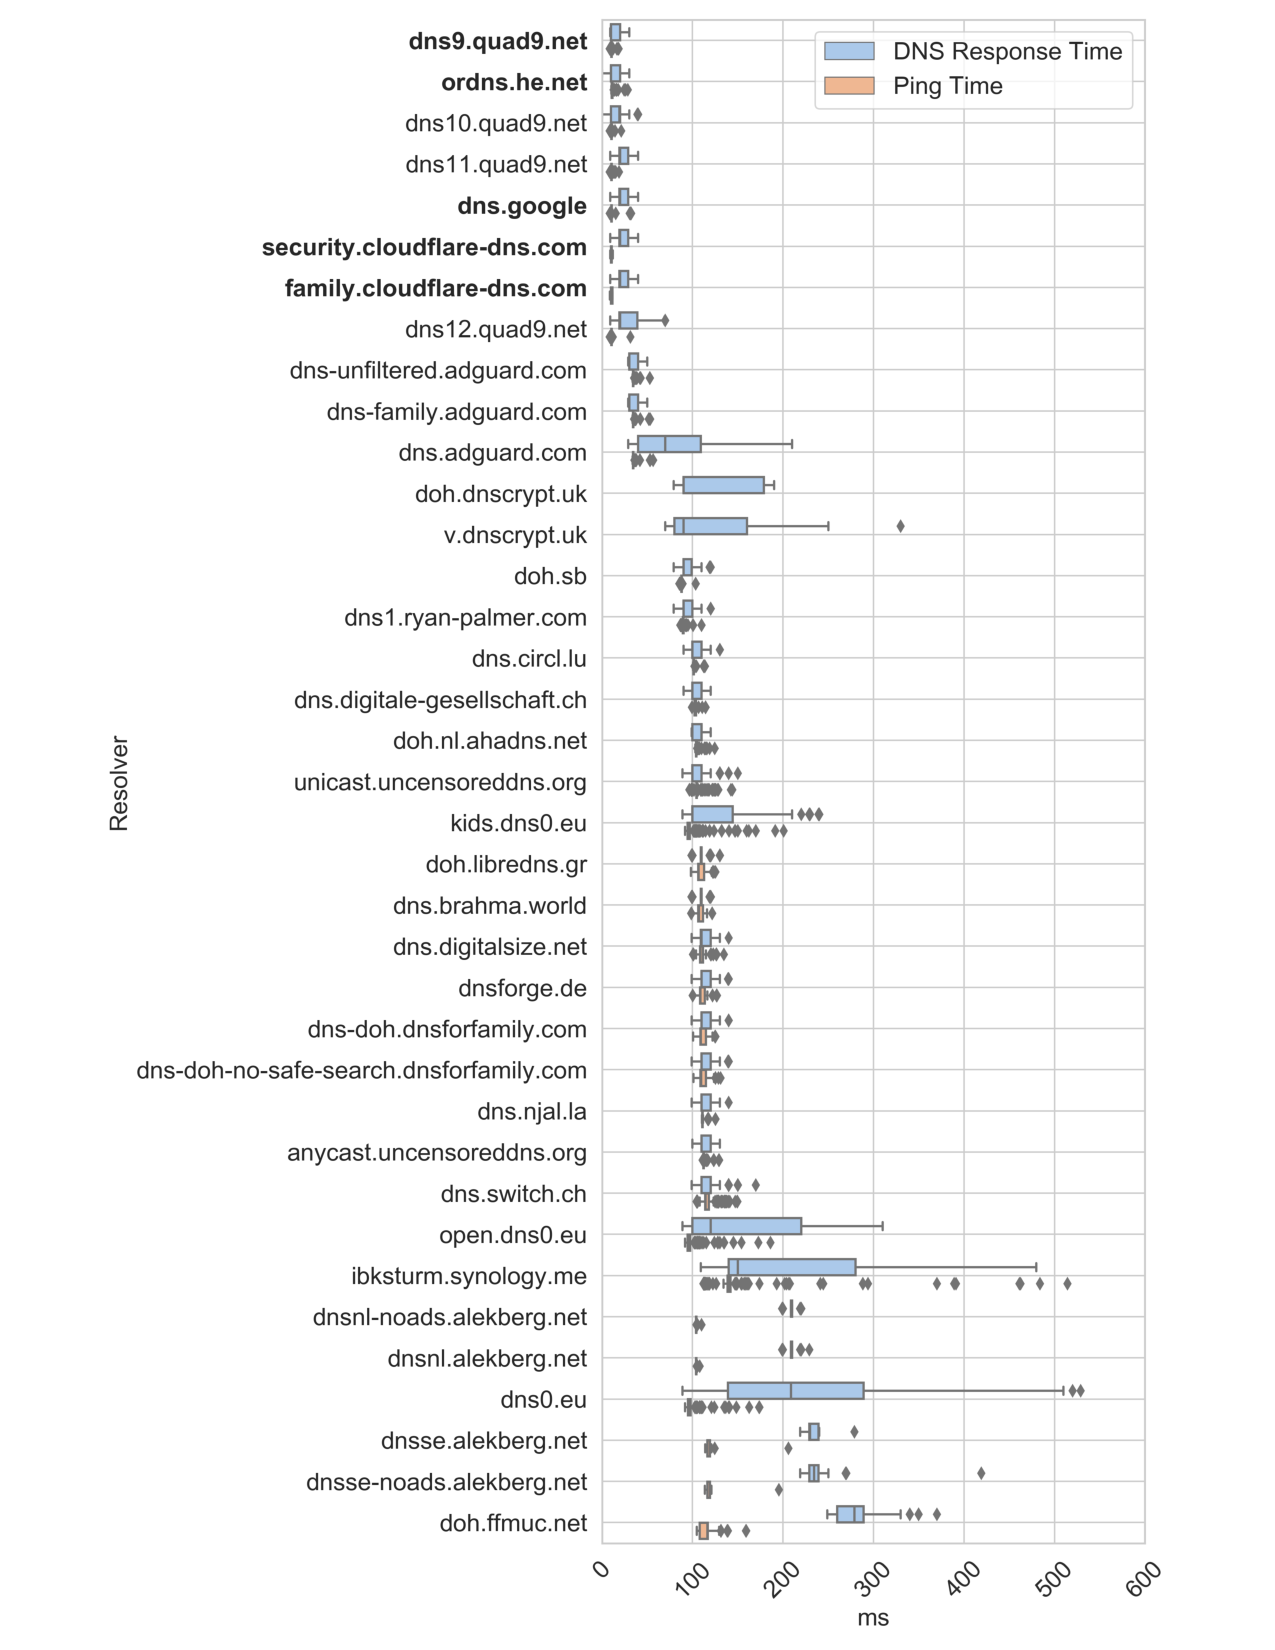
\includegraphics[width=\textwidth]{figures/ohio_eur.pdf}
\caption{Ohio EC2.}
\end{subfigure}
%
\hfill \\
\begin{subfigure}[b]{0.4\textwidth}
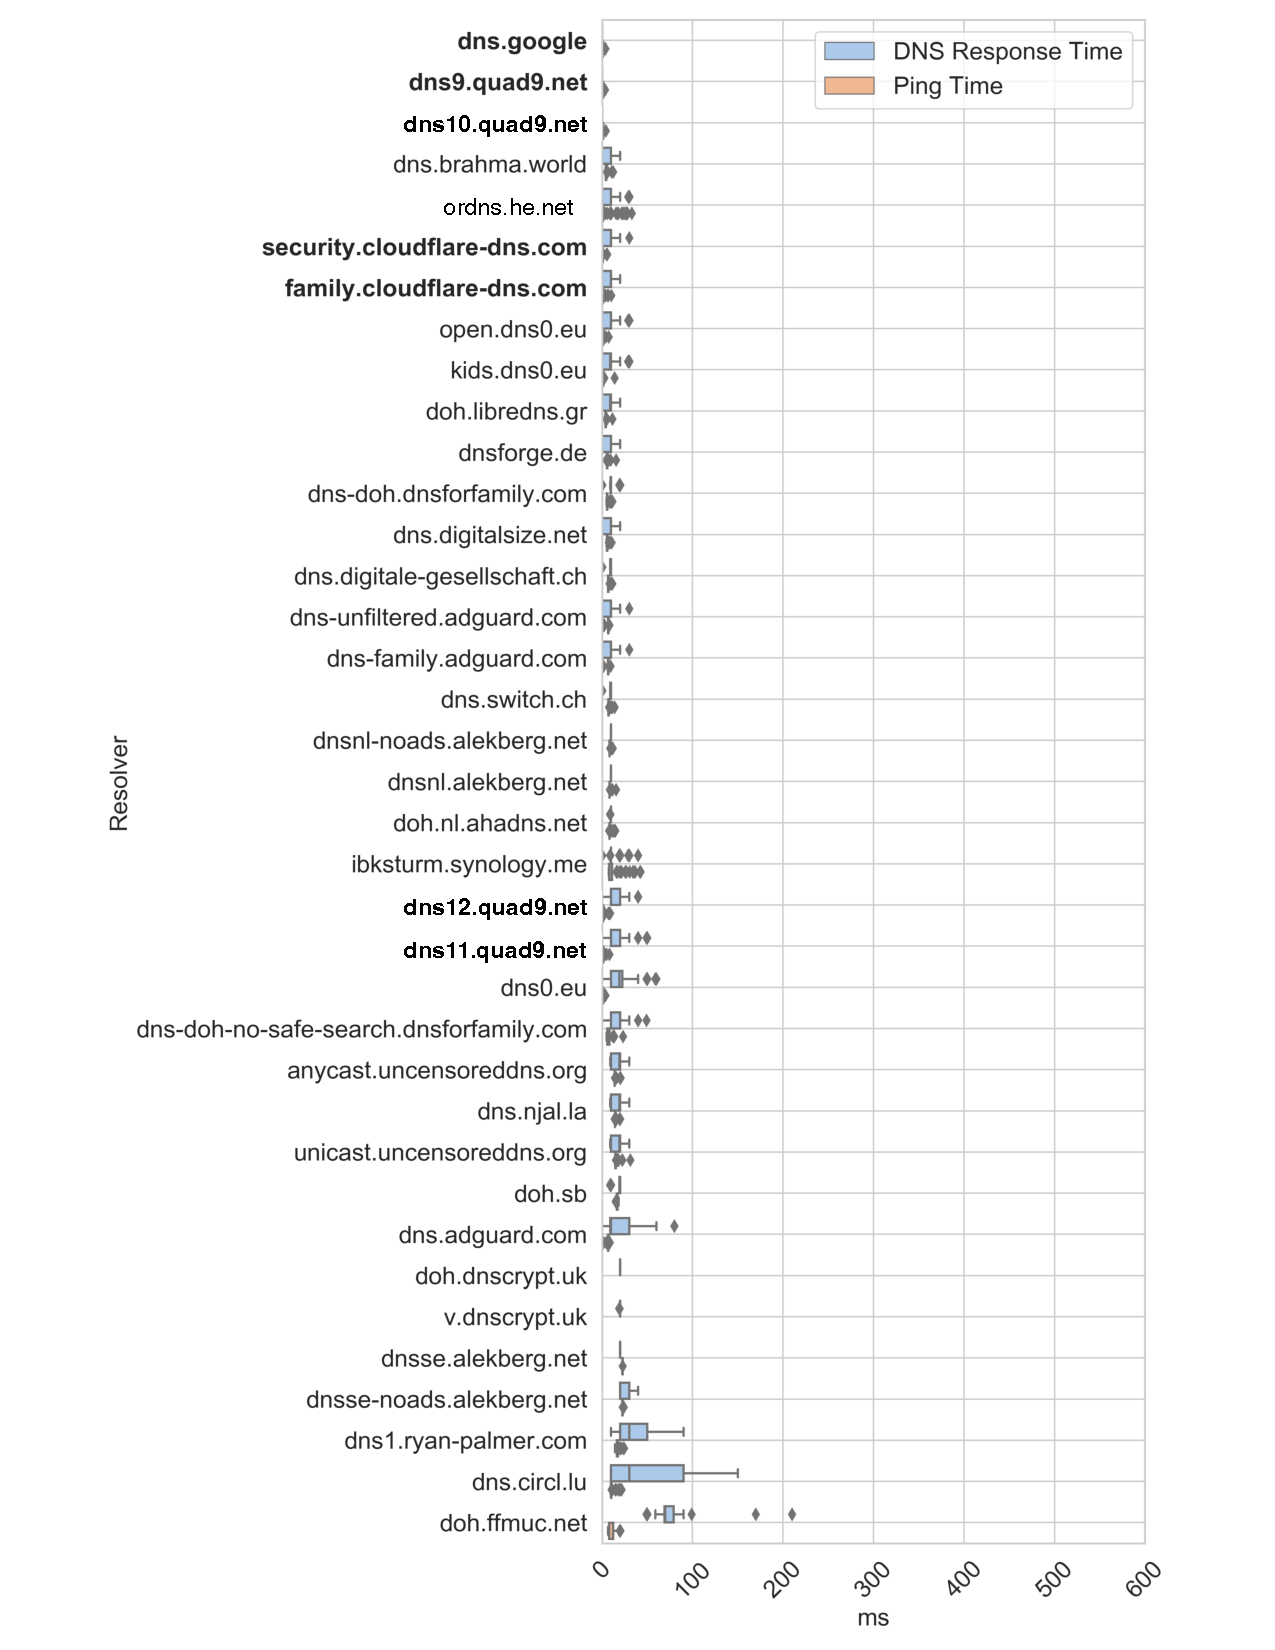
\includegraphics[width=\textwidth]{figures/frankfurt_eur.pdf}
    \caption{Frankfurt EC2 (Local).}
\end{subfigure}
%
\begin{subfigure}[b]{0.4\textwidth}
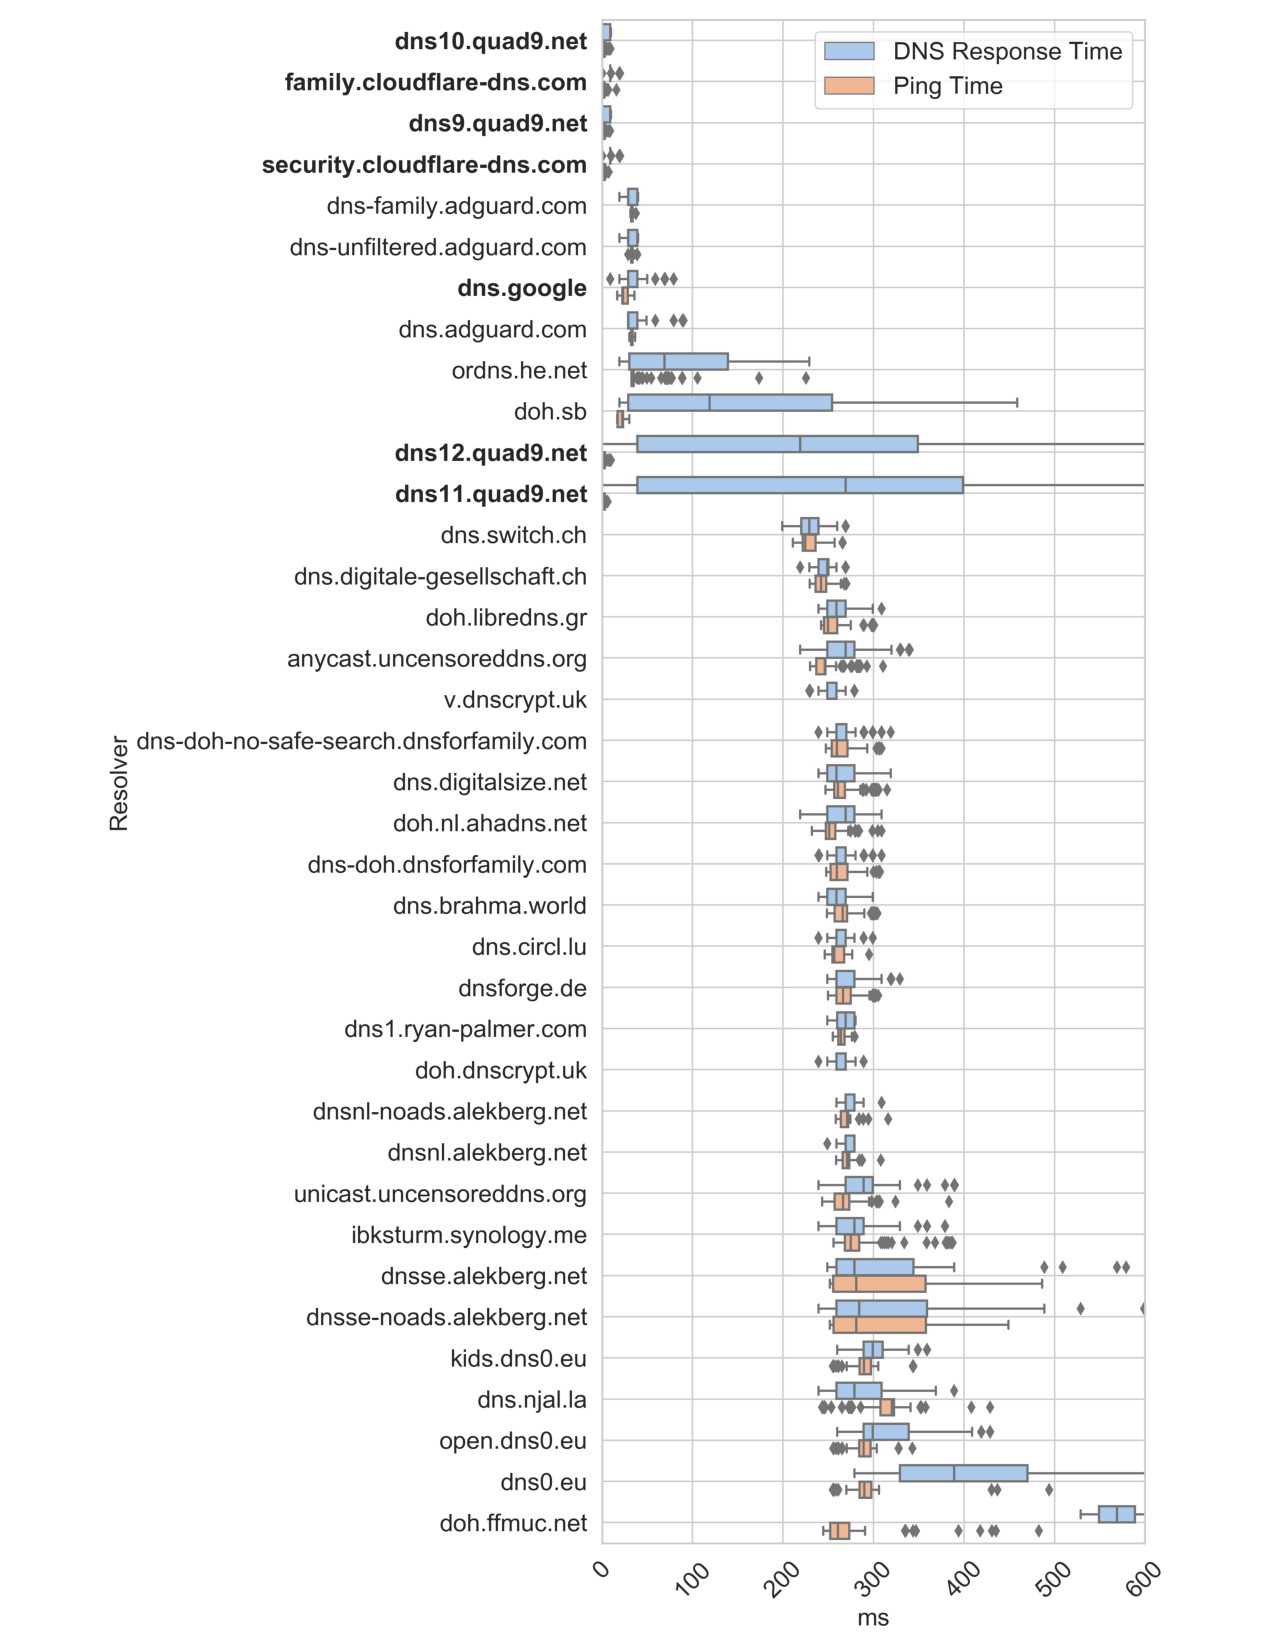
\includegraphics[width=\textwidth]{figures/seoul_eur.pdf}
\caption{Seoul EC2.}
\end{subfigure}
\caption{The DNS response time and ICMP ping time distributions for
    encrypted DNS resolvers located in Europe, measured from global vantage points.
    Mainstream resolvers are shown in boldface across all three
    sub-figures.}
\label{fig:dns-europe}
\end{figure*}
\begin{figure*}[h!]
\centering
%
\begin{subfigure}[b]{0.4\textwidth}
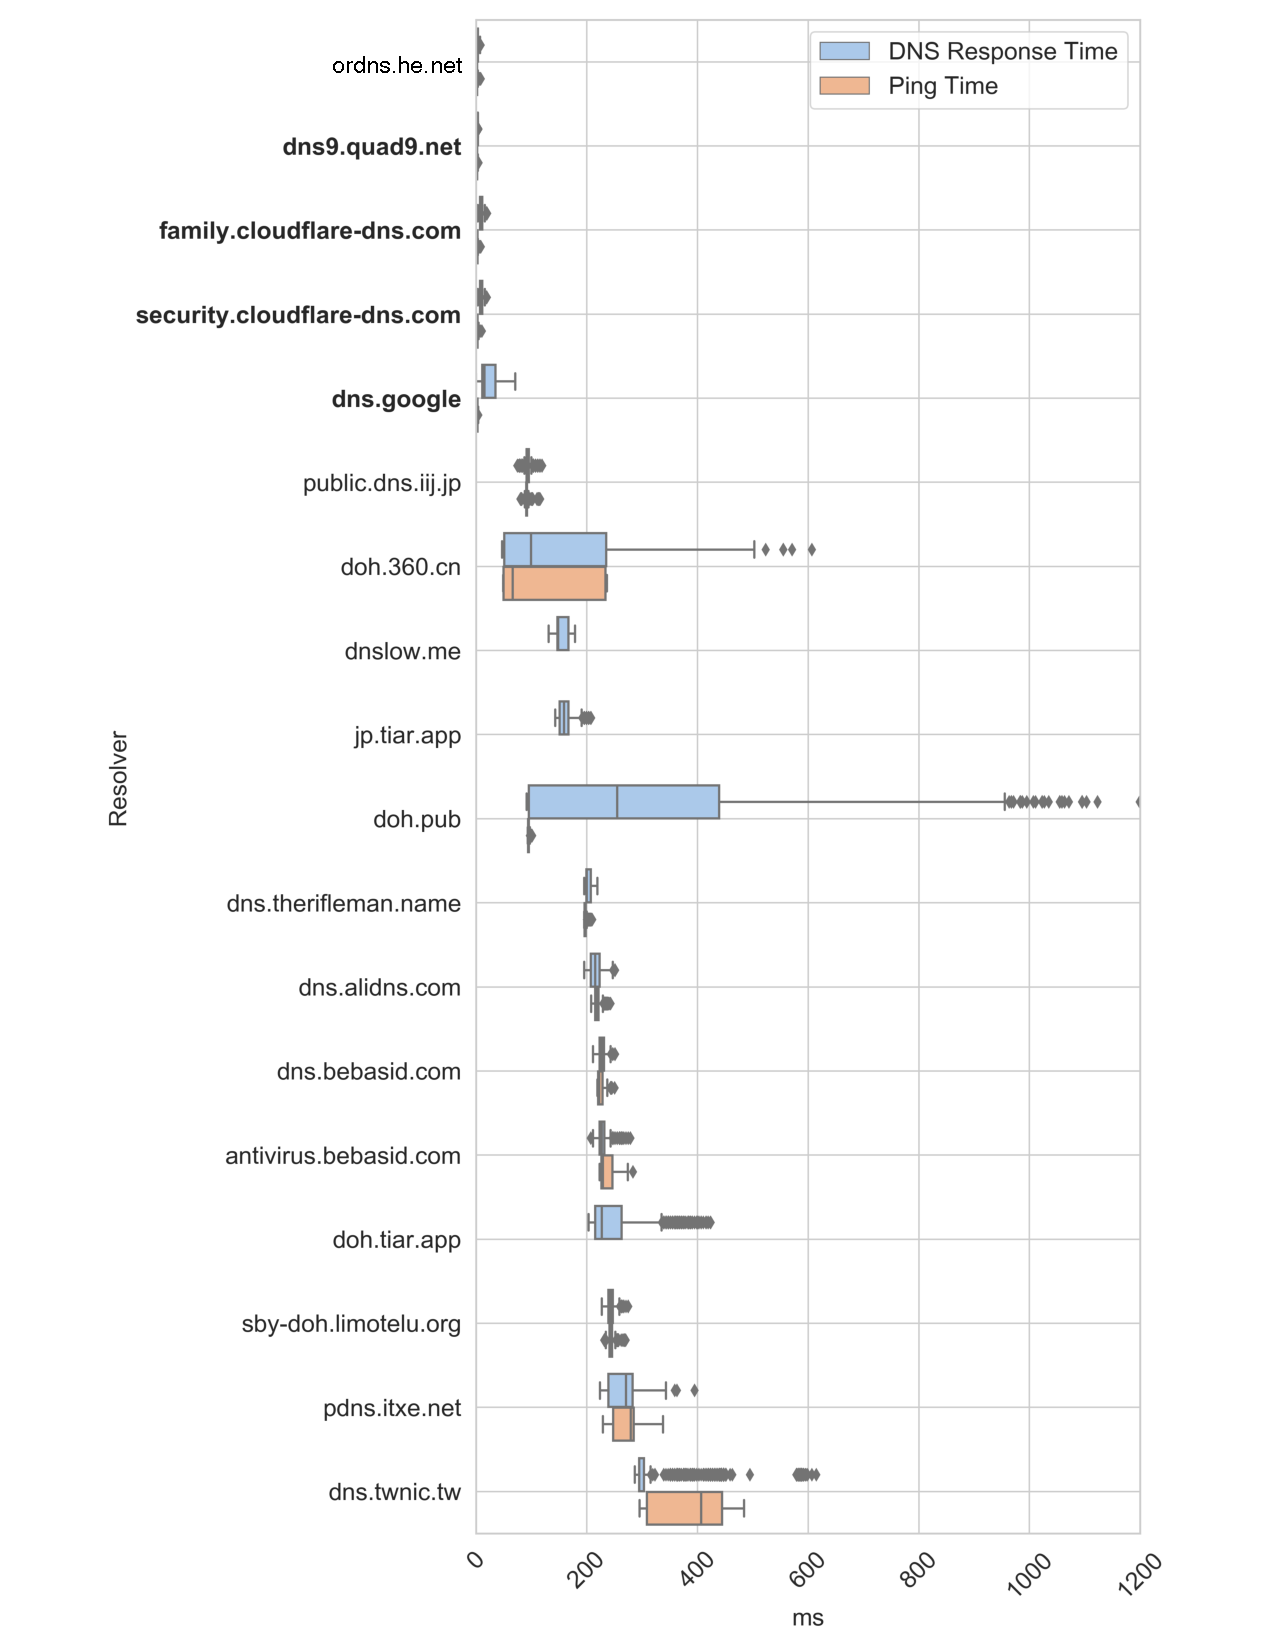
\includegraphics[width=\textwidth]{figures/poah_asia.pdf}
\caption{U.S. Home Networks}
\end{subfigure}
%
\begin{subfigure}[b]{0.4\textwidth}
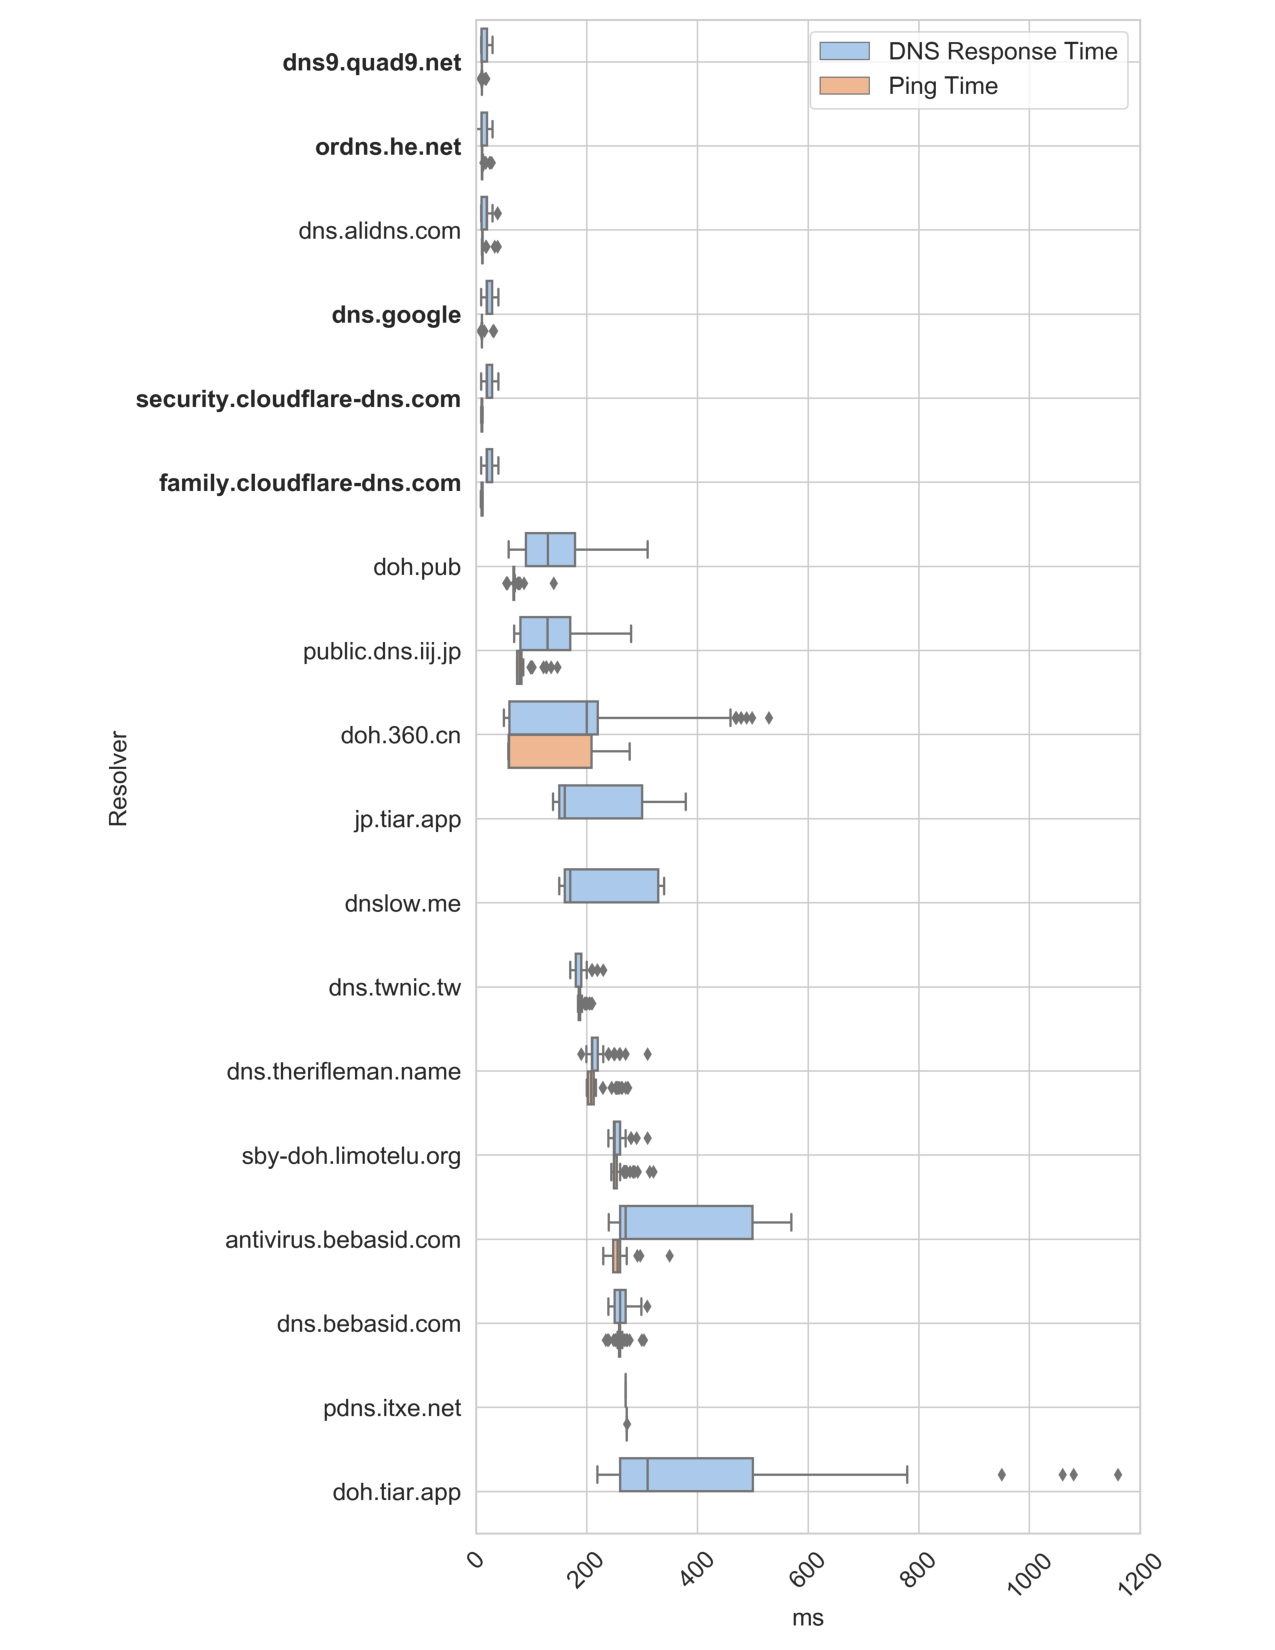
\includegraphics[width=\textwidth]{figures/ohio_asia.pdf}
\caption{Ohio EC2.}
\end{subfigure}
%
\hfill \\
\begin{subfigure}[b]{0.4\textwidth}
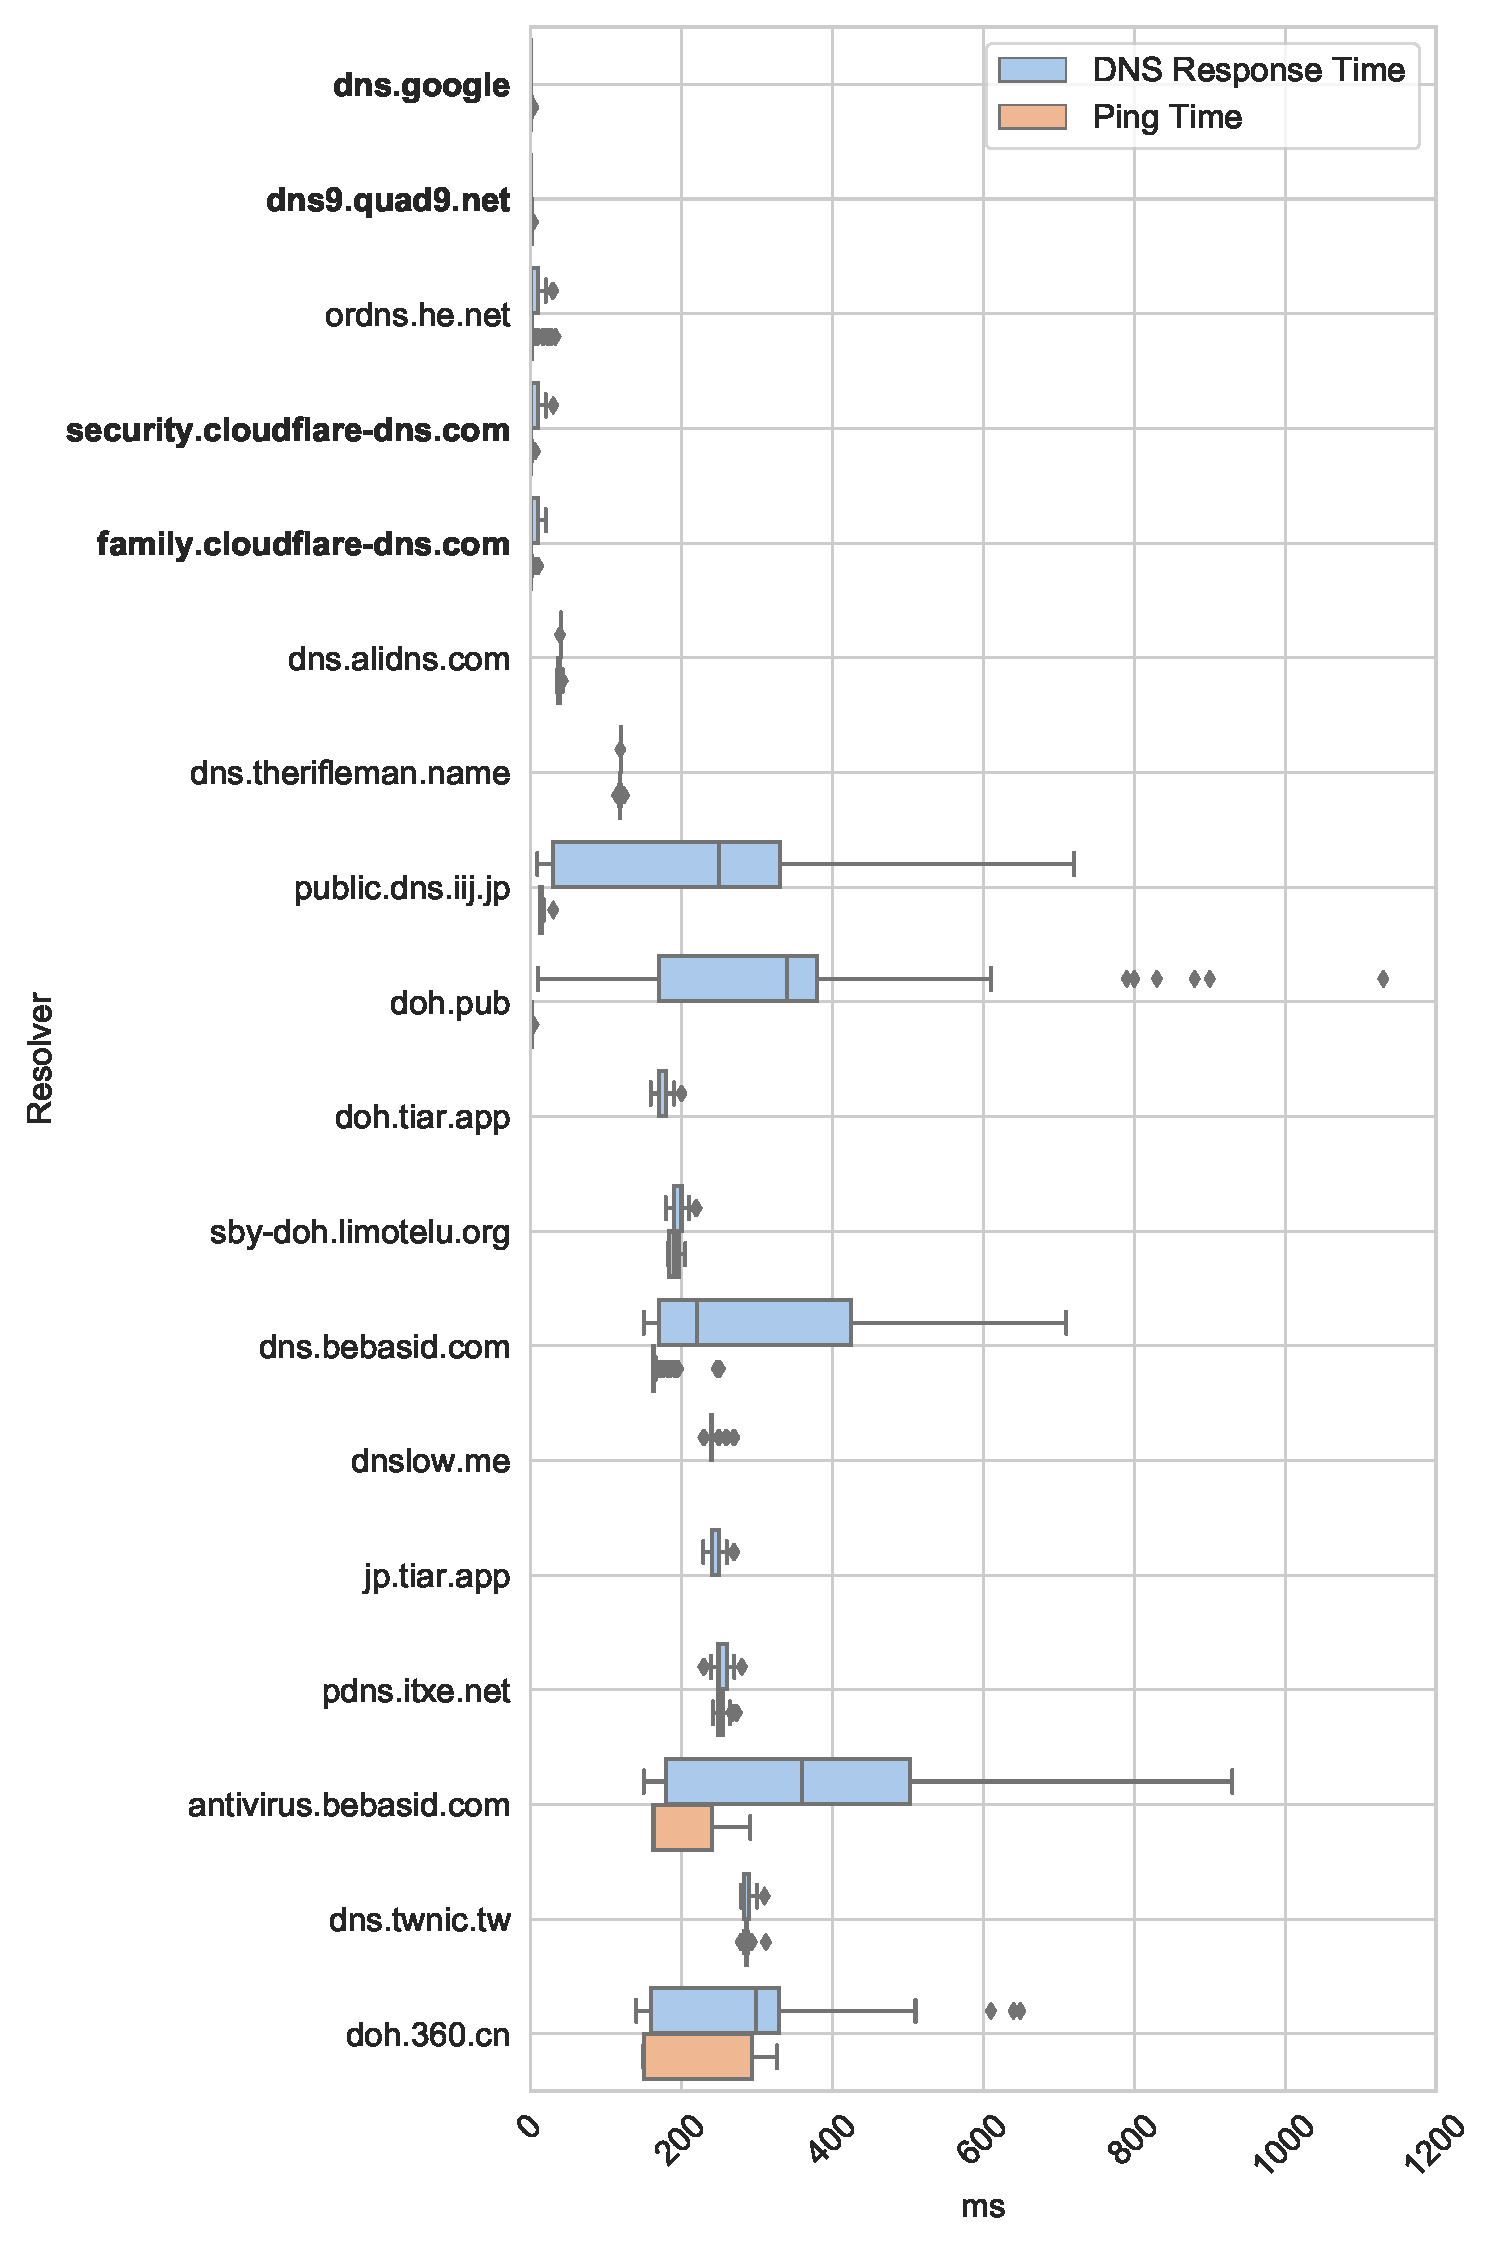
\includegraphics[width=\textwidth]{figures/frankfurt_asia.pdf}
    \caption{Frankfurt EC2.}
\end{subfigure}
%
\begin{subfigure}[b]{0.4\textwidth}
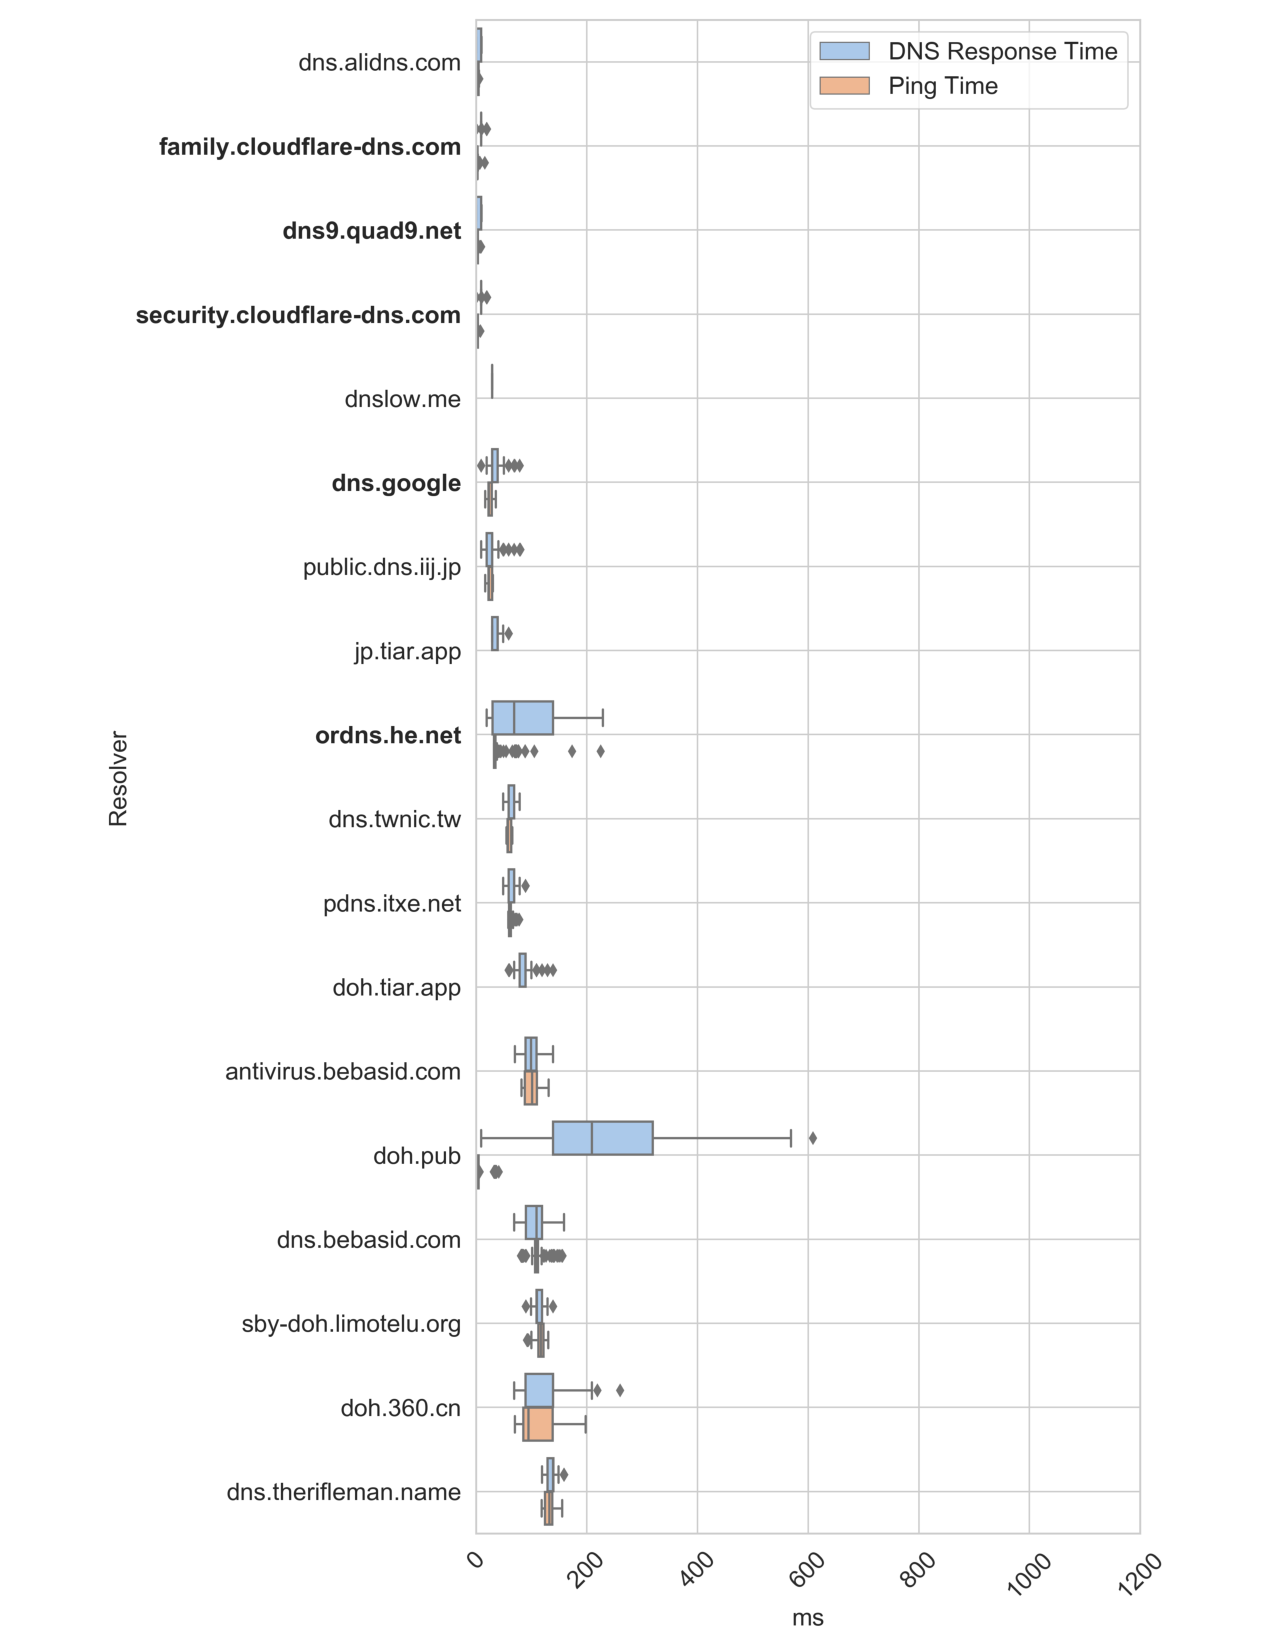
\includegraphics[width=\textwidth]{figures/seoul_asia.pdf}
    \caption{Seoul EC2 (Local).}
\end{subfigure}
\caption{The DNS response time and ICMP ping time distributions for
    encrypted DNS resolvers located in Asia, measured from global vantage points.
    Mainstream resolvers are shown in boldface across all three
    sub-figures.}
\label{fig:dns-asia}
\end{figure*}
